%Dies ist die Hauptseite des Dokumentes. Es werden u. a. alle Kapitel,
%Einstellung im Header eingebunden.
%Veränderungen müssen in folgenden Dateien vorgenommen werden:
      %- config.tex
      %- einzelne Kapitel (evtl. erweitern)

\input{common/layout.tex}          % Diese Datei enthält alle
                                          % Layouteinstellungen
\newcommand{\dokumentTitel}{Angebot}
% Definition von globalen Parametern, die derzeit auf der Titelseite und in der
% Kopfzeile verwendet werden. Der in <> gesetzte Text ist zu verändern.

\newcommand{\praktikumTitel}{<Titel des Praktikums>}
\newcommand{\projektTitel}{<Titel des Teilprojektes>}
\newcommand{\institut}{
	<Name des Instituts>\\
	<Name des Institutsleiters>\\
	<Straße und Hausnummer>\\
	<Postleitzahl und Ort>\\
}
\newcommand{\institutsLogo}{common/ISF_Logo.pdf}
\newcommand{\betreuer}{<Name>}


%------Beginn des Gesamtdokumentes----------------------------------------------
\begin{document}

%------Eingebundene Seiten, Verzeichnisse bzw. Kapitel--------------------------
\include{common/titelseite}                      % Titelseite

\tableofcontents                          % Inhaltsverzeichnis wird automatisch
                                          % generiert
\listoffigures                            % ebenso das Abbildungsverzeichnis

%----Kapitel des Feinentwurfs, die mit Inhalt zu füllen sind--------------------
%!TEX root = ../Systementwurf.tex

\chapter{Einleitung}

\NewsGenie ist der persönliche Nachrichtensprecher. Immer auf dem neuesten
Stand und begierig darauf, die Fragen seiner Nutzer zu beantworten.
"`Was gibt es Neues in Russland?"', "`Wie hat Eintracht
Braunschweig gespielt?"', "`Wie alt ist Angela Merkel?"' - \NewsGenie
versteht seinen Benutzer ohne Tastatur, Suchmaske oder Bildschirm sondern in
völlig normaler Sprache.

Als Thin-Client-Server-Anwendung wird \NewsGenie so realisiert, dass der
Nutzer mittels eines kleinen und günstigen Clients auf das System
zugreifen und seine Anfragen stellen kann. Dabei hat er die Möglichkeit nach
Nachrichten aus einem Bereich, wie \glqq Technologie\grqq\, einem bestimmten aktuellen Thema, wie der Ukraine, sowie nach Fakten,
z.B. dem Alter einer Person des öffentlichen Lebens, zu suchen.

Um dies zu realisieren, wird dem Server eine maßgebliche Rolle zuteil. Dieser verarbeitet die Anfragen der verschiedenen Clients, 
erfasst parallel die einzelnen Nachrichtenartikel von den in der Datenbank
hinterlegten Newsseiten und stellt den Nutzern ein Webinterface zur Verfügung.

Der Server basiert auf einer 3-Schichten-Architektur aus
Benutzerschnittstelle, System- und Persistenzschicht und wird in Java
entwickelt.
Die Benutzerschnittstelle besteht auf der Serverseite aus dem Webinterface, das mit Hilfe des Play-Frameworks\footnote{Mit dem quelloffenen Play-Framework kann man einfach ressourcenschonende Web-Applikationen in Java und Scala entwickeln. \url{http://www.playframework.com/}} realisiert wird.
Die Systemschicht stellt die Kernfunktionalität des Servers bereit, das Annehmen von Anfragen, deren Verarbeitung mit Hilfe von "`Natural Language Processing"'\footnote{Stanford CorNLP, eine Sammlung von Sprachanalysetools. Verwendet werden der Part-of-Speech tagger (POS) und der Named Entity Recognizer (NER), \url{http://nlp.stanford.edu/software/corenlp.shtml}} und außerdem den Crawler, welcher regelmäßig die hinterlegten Newsseiten nach neuen Artikeln durchsucht und in der Persistenzschicht, einer Datenbank realisiert mit einem Virtuoso\footnote{OpenLink Virtuoso ist ein quelloffenes Datenbanksystem, das die Funktionalität vieler verschiedener Datenbankparadigmen kombiniert. Wird hier als Triple-Store verwendet. \url{http://virtuoso.openlinksw.com/dataspace/doc/dav/wiki/Main/}} Triple-Store, speichert. 
Die Datenbank ist außerdem mit einem Lucene-Index versehen.

%
%Die Benutzerschnittstelle besteht auf der Serverseite aus dem Webinterface.
%In diesem kann sich der Benutzer registrieren und nach einem Login Textanfragen stellen
%und seine Nachrichtenquellen verwalten. 
%Weiterhin besteht die Möglichkeit, sein Passwort zu ändern oder wiederherzustellen und 
%seinen Account zu löschen. Administratoren können außerdem in die Sicht von anderen
%Benutzern wechseln und diese löschen. Das Webinterface wird mit Hilfe des Play-Frameworks realisiert.
%
%Die Systemschicht stellt die Kernfunkionalitäten des Servers bereit. Der
%Management-Handler nimmt alle Anfragen von Clients und aus dem Webinterface entgegen 
%und koordinert die weiteren Schritte. Handelt es sich dabei ausschließlich um eine Anfrage nach Daten,
%wie zum Beispiel bei einem Login-Versuch, wo geprüft werden muss, ob ein Nutzername registriert ist, 
%werden diese Informationen aus der Datenbank gesucht und die Anfrage so beantwortet. Handelt es sich 
%jedoch um eine Anfrage nach Neuigkeiten, besteht diese aus natürlicher Sprache und muss zunächst interpretiert werden.
% Hierzu wird die eingegangene Anfrage
% durch "`Natural Language Processing"' analysiert und durch
%unser eigenes Analysetool geschickt, welches die enthaltenen Wörter in einen Kontext setzt.
%Anschließend werden die am Besten zur Anfrage passenden Artikel aus der Datenbank gesucht und das
% Ergebnis wieder in einen natürlichen Satz umgewandelt.
%Außerdem beinhaltet die Systemschicht den Crawler, welcher die in der Datenbank
%hinterlegten Newsseiten regelmäßig nach neuen Artikeln durchsucht.
%
%Die Persistenzschicht beinhaltet einen Virtuoso-Triplestore, der als Datenbank dient, 
%sowie einen Lucene-Index zur effizienten Volltextsuche. 
%In Virtuoso werden die Daten der Benutzer sowie Feeds und deren beinhaltete Artikel gespeichert.

Alle Schichten kommunizieren mit Hilfe des Akka-Frameworks\footnote{Akka ist ein Framework zur Entwicklung fehlertoleranter, verteilter Java- und Scala Anwendungen, basierend auf dem Aktoren-Modell. \url{http://akka.io/}}, welches einen sicheren,
asynchronen Datenaustausch ermöglicht.

Aus der genannten Aufteilung resultieren die in Abb. \ref{komponenten}
dargestellten Komponenten.

In den nachfolgenden Abschnitten wird die Implementierung \NewsGenie vorgestellt. Zunächst die Komponentenaufteilung, gefolgt von Implementierungsdetails wie den einzelnen Funktionen und dem Datenmodell.

\begin{figure}[h]
\centering
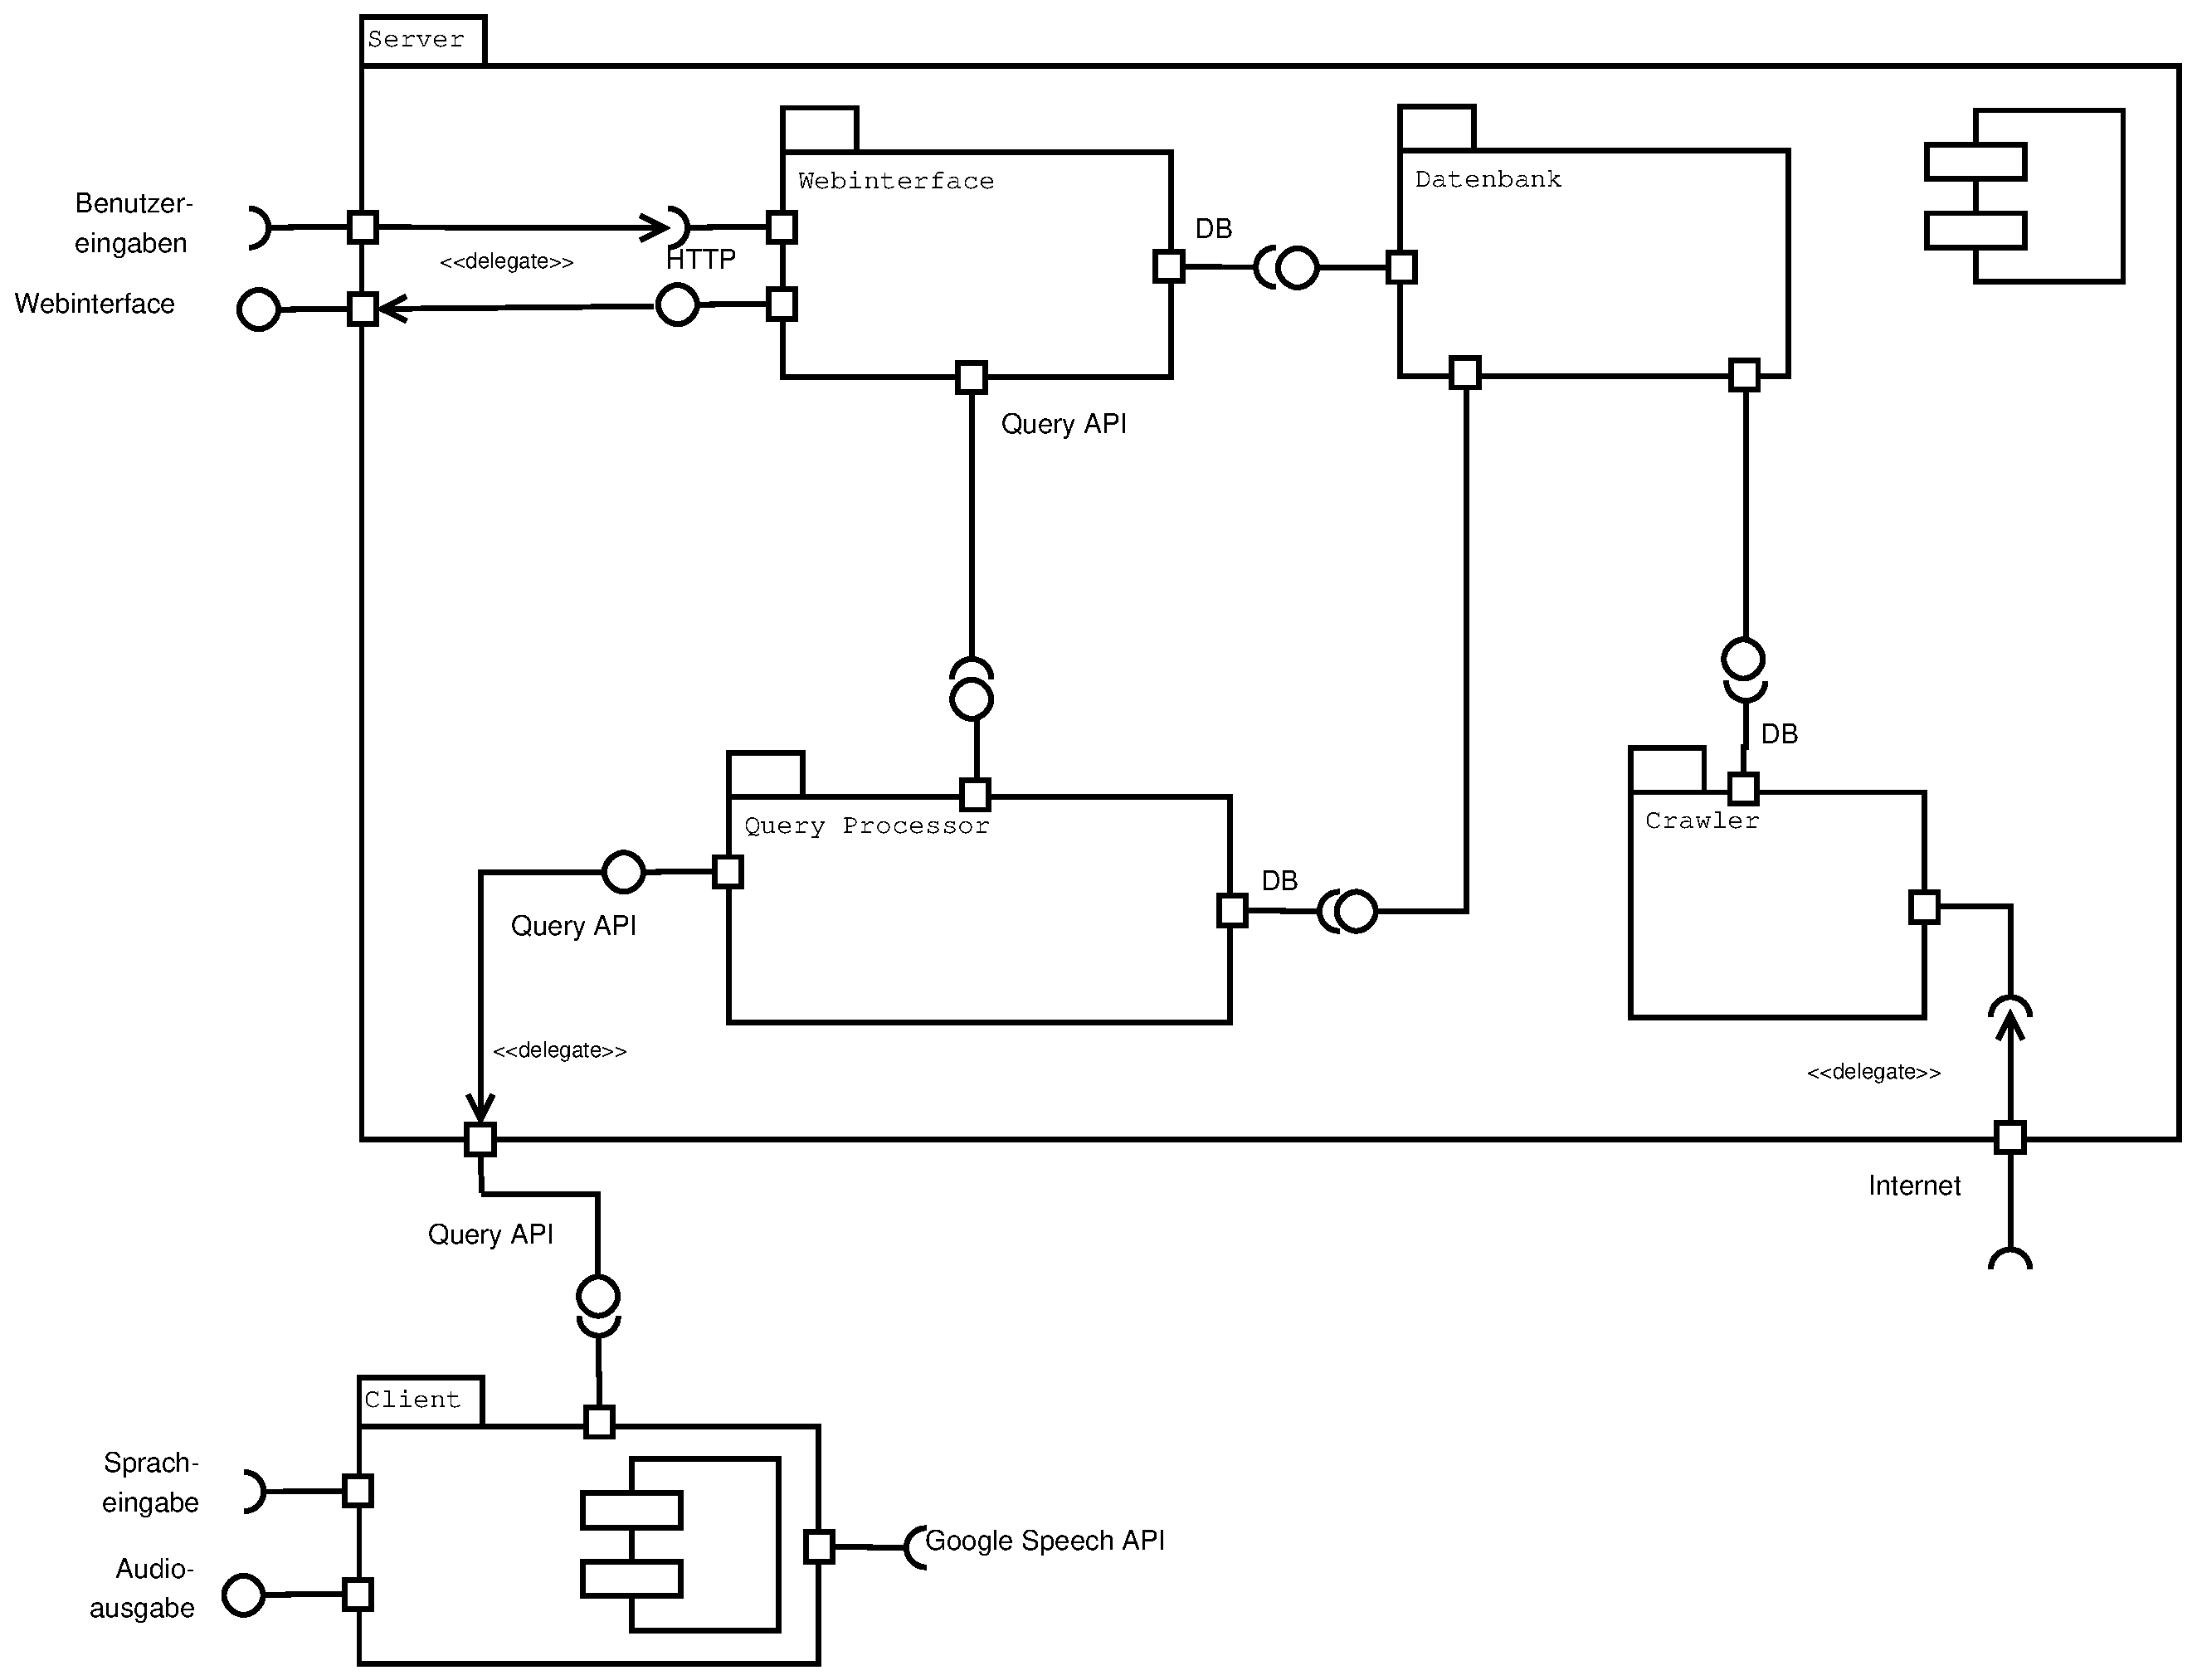
\includegraphics[width=1\textwidth]{Systementwurf/05_implementierungsentwurf/komponenten}
\caption{Komponentendiagramm, \textit{Komponentenaufteilung von \NewsGenie}
\label{komponenten}}
\end{figure}

\FloatBarrier
\section{Projektdetails}

Um wichtige Aspekte von \NewsGenie genauer zu erläutern, werden in diesem
Kapitel verschiedene Funktionen der Anwendung aufgeführt und beschrieben. In den folgenden
Unterkapiteln werden das Registrieren, die Anmeldung am Webinterface, das Hinzufügen von Feeds
 und die Interaktion zwischen Benutzer und Client genauer erklärt.

\subsection{Registrieren und Anmelden}

Die folgenden Aktivitätsdiagramme~\ref{1.2}~und~\ref{1.3} beschreiben den Workflow bei der Registrierung
 und Anmeldung eines Nutzers. Will
sich ein Nutzer registrieren um \NewsGenie zu nutzen, so muss er im Webinterface
den entsprechenden Registrierungs-Button anklicken. Dadurch wird ihm vom System
die Seite angezeigt, auf der er seinen gewüschten Benutzernamen und sein selbst
gewähltes Passwort sowie seine E-Mail-Adresse in Textfelder eintragen kann.
Nachdem der Nutzer seine Eingaben bestätigt hat, legt das System
seine Daten in der Datenbank ab, sofern sie nicht schon vergeben waren.
 Nun kann der Nutzer sich am Client und im
Webinterface anmelden. Über den Client kann er anschließend Anfragen stellen
oder über das Webinterface seine Einstellungen verwalten bzw. eine Textanfrage
stellen.

\begin{figure}[h]
\centering
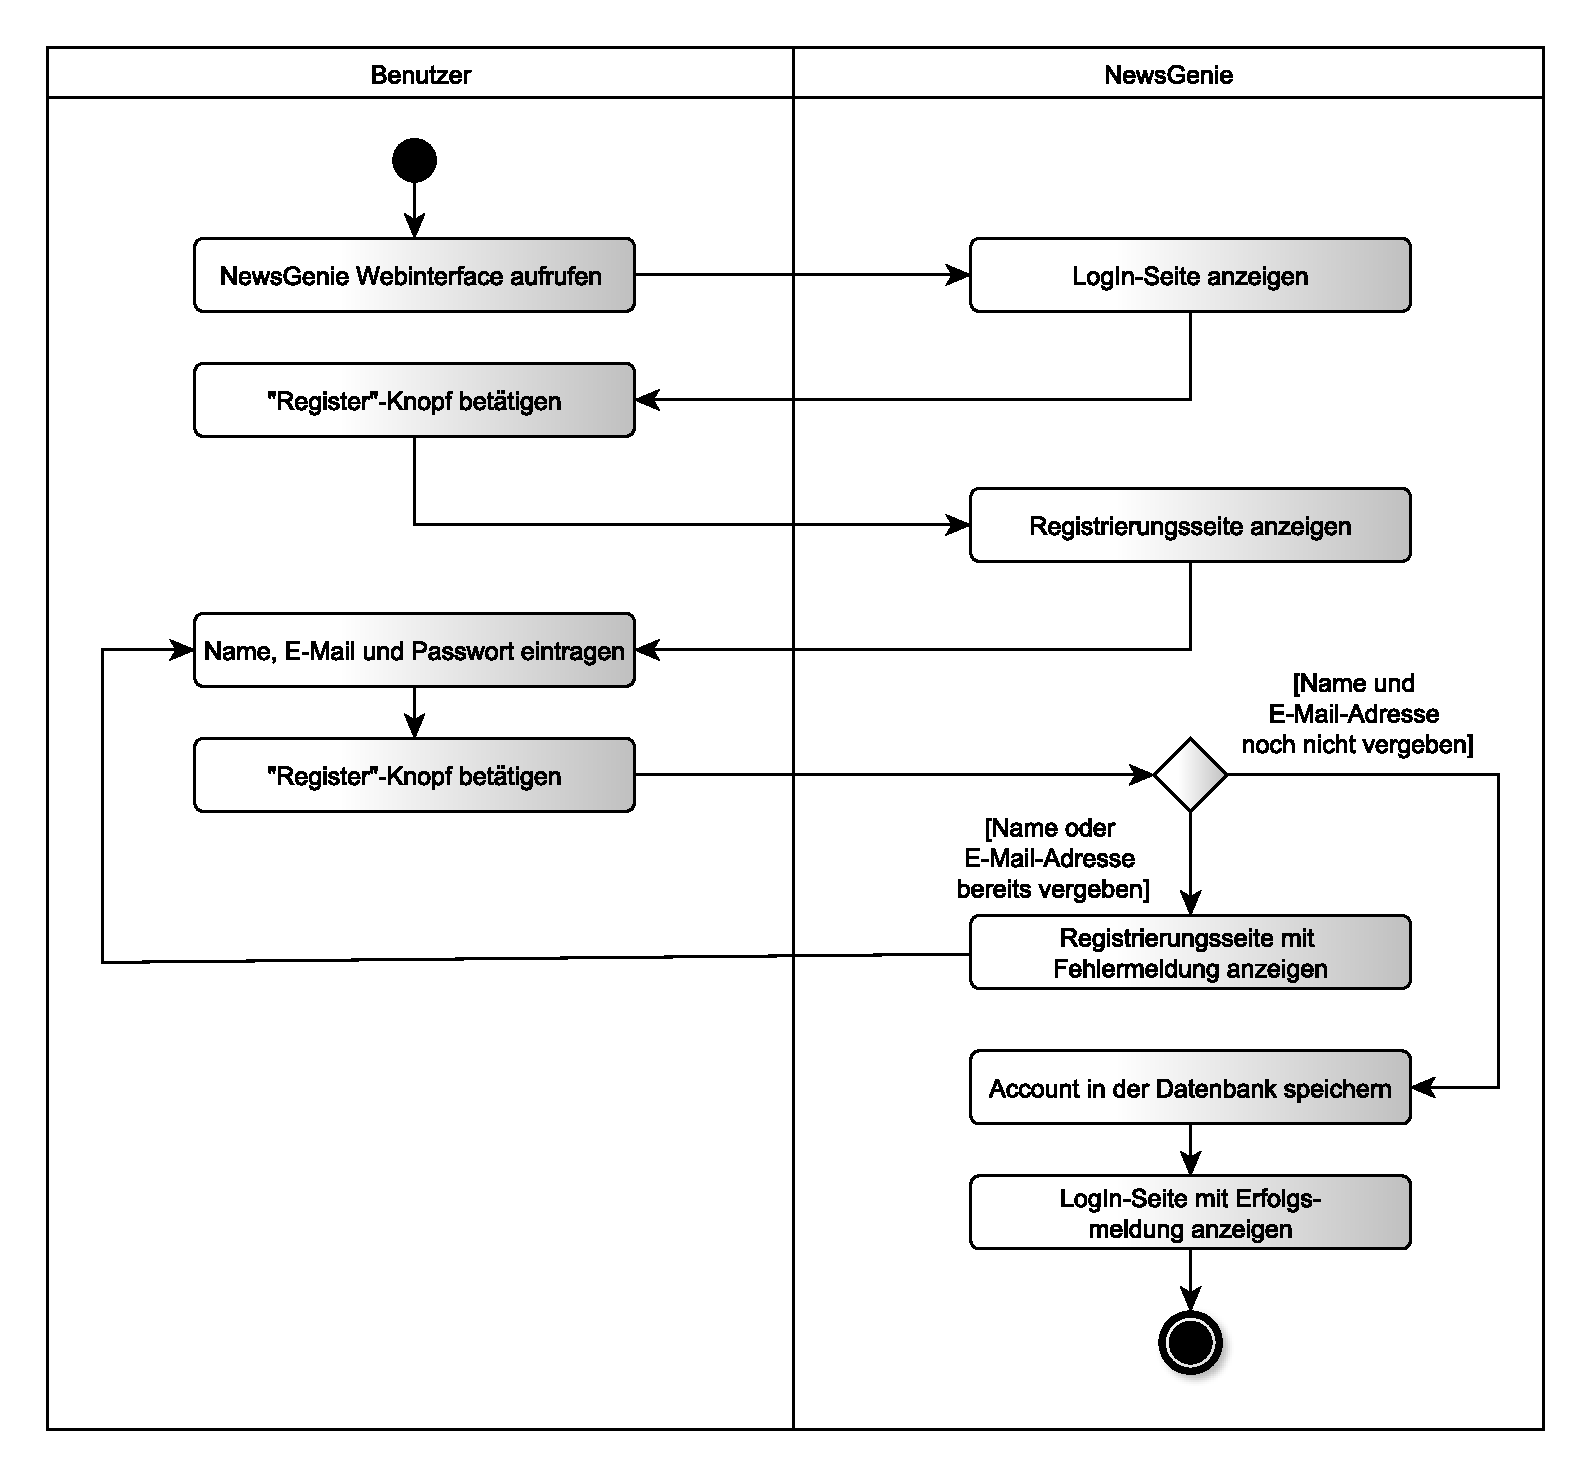
\includegraphics[width=1\textwidth]{Systementwurf/01_einleitung/register.eps}
\caption{Aktivitätsdiagramm, \textit{Registrierung bei \NewsGenie}
\label{1.2}}
\end{figure}

\begin{figure}[h]
\centering
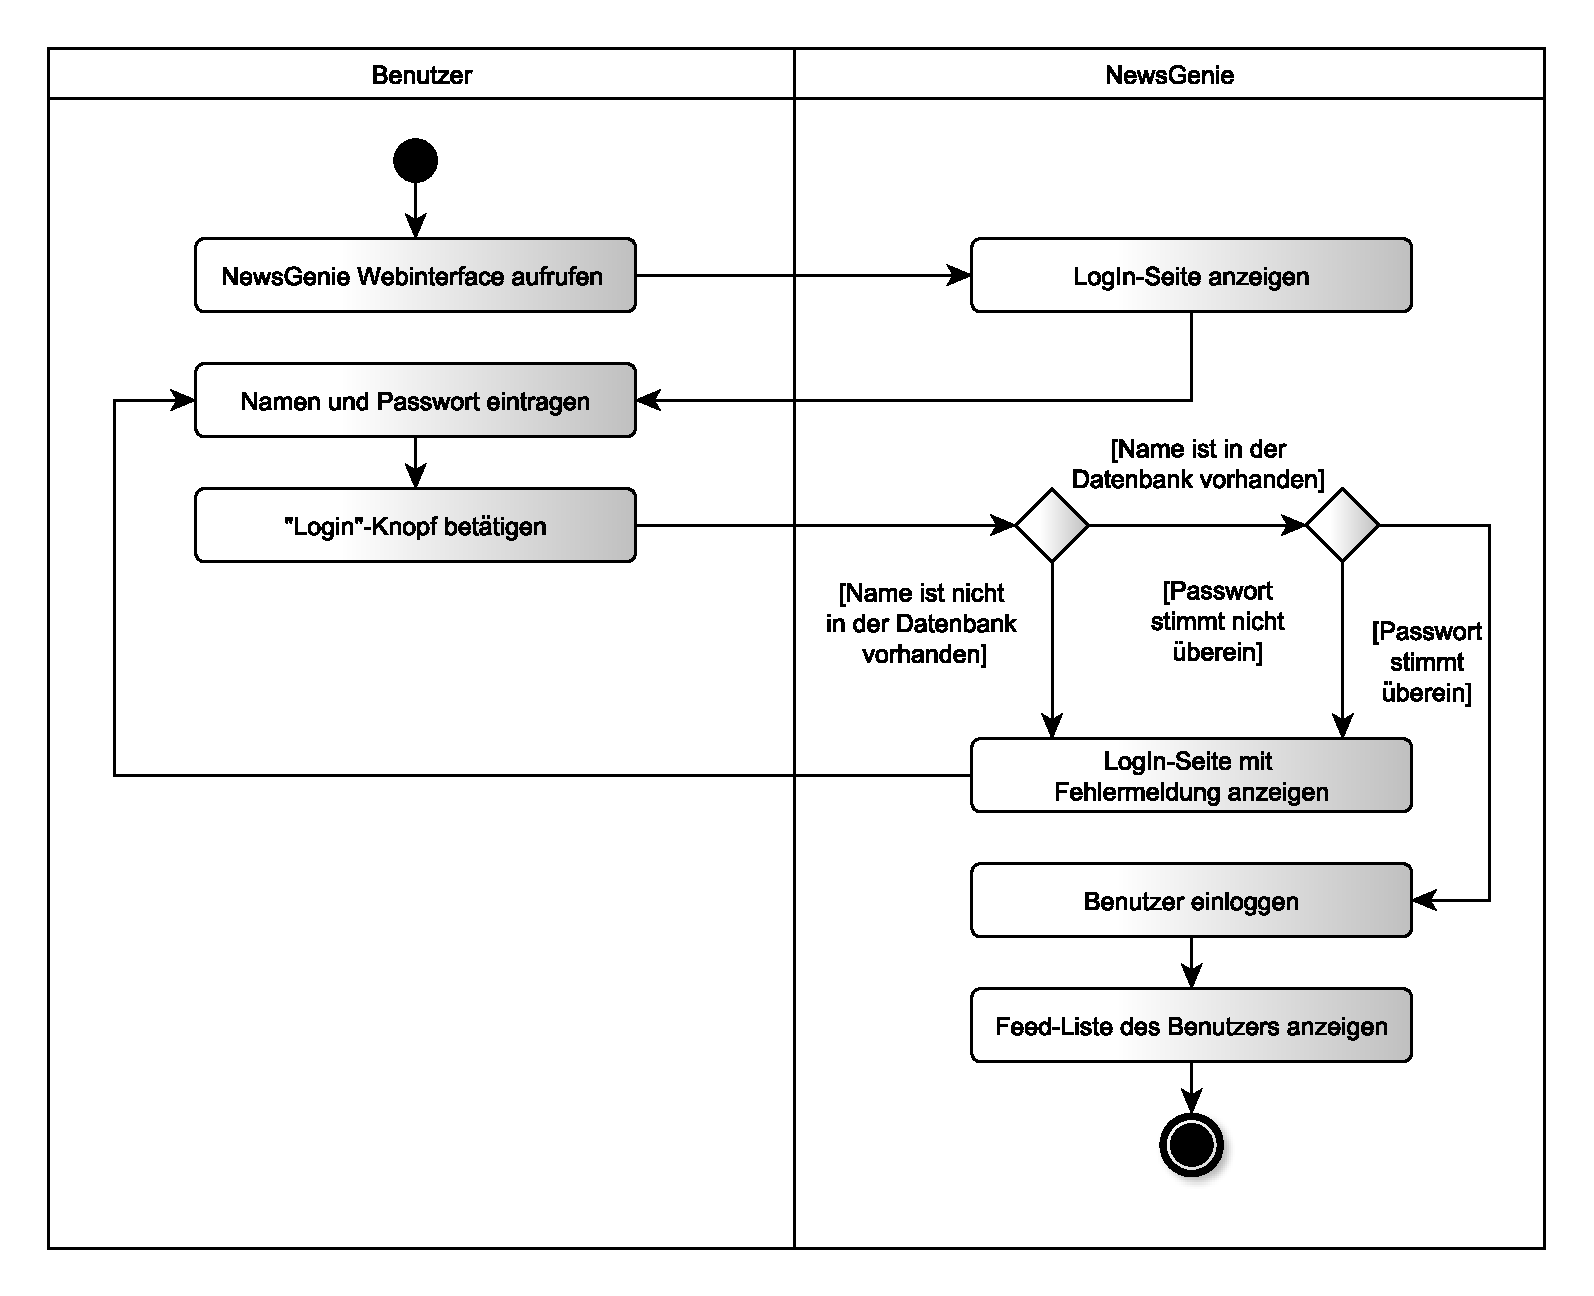
\includegraphics[width=1\textwidth]{Systementwurf/01_einleitung/weblogin.eps}
\caption{Aktivitätsdiagramm, \textit{Anmeldung am Webinterface}
\label{1.3}}
\end{figure}

\subsection{Feeds hinzufügen}

Sobald ein Benutzer sich am Webinterface eingeloggt hat, besteht für ihn die Möglichkeit, 
seine Feeds zu verwalten. Im nachfolgenden Aktivitätsdiagramm~\ref{1.4} wird dargestellt,
wie ein Benutzer neue Feeds abonnieren kann. Es reicht dazu aus, die URL des hinzuzufügenden 
Feeds in das dazu vorgesehene Textfeld einzugeben und die Eingabe per Knopfdruck zu bestätigen.
Das System prüft nun ob unter der angegebenen URL tatsächlich ein Feed zu finden ist und gibt sonst
eine Fehlermeldung aus. Falls der Feed existiert, wird er in der Datenbank gespeichert, falls dies noch nicht der Fall ist, und der Benutzer wird ihm als Abonnent zugeordnet.

\begin{figure}[h]
\centering
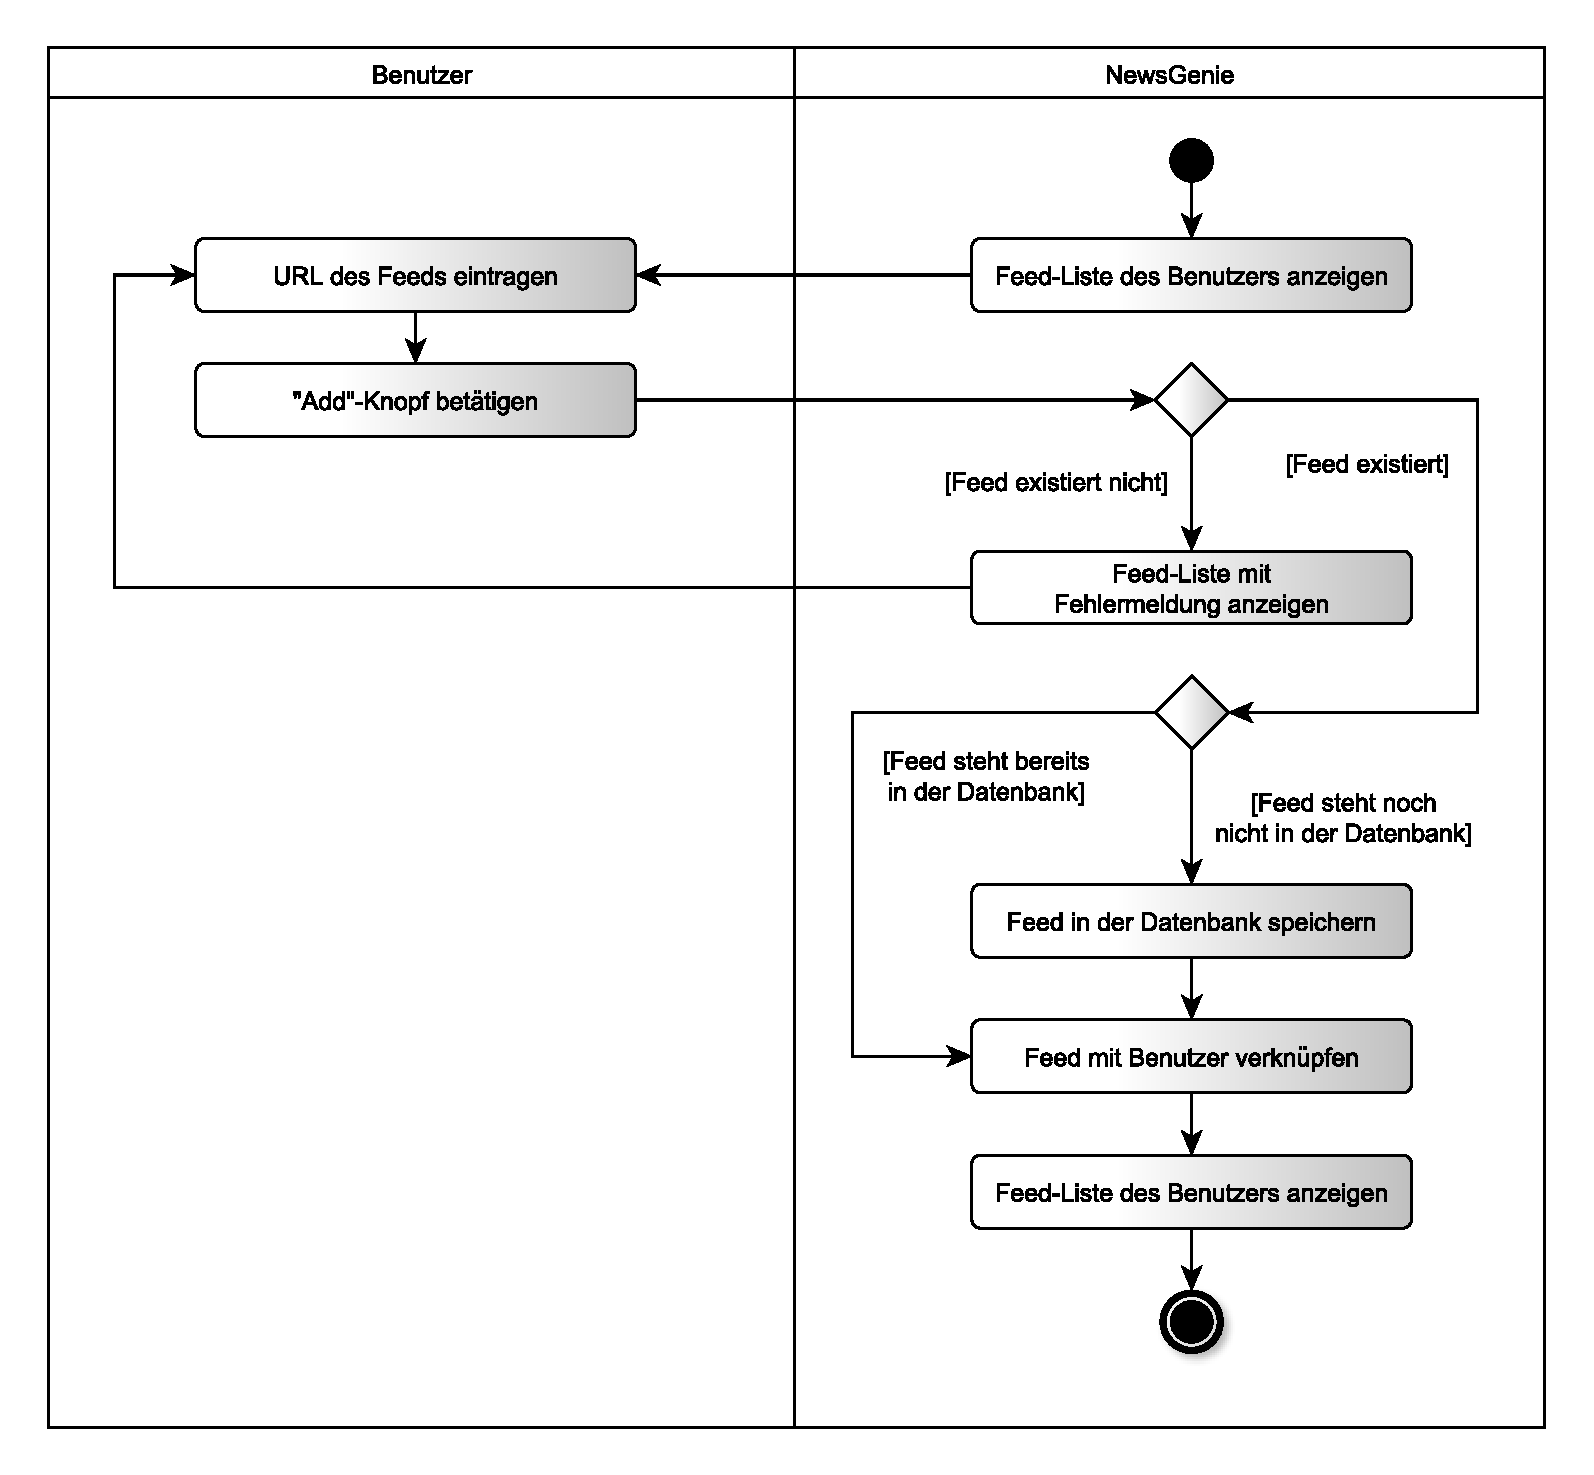
\includegraphics[width=1\textwidth]{Systementwurf/01_einleitung/addfeed.eps}
\caption{Aktivitätsdiagramm, \textit{Hinzufügen von Feeds}
\label{1.4}}
\end{figure}

\pagebreak[3]

\subsection{Interaktion zwischen Benutzer und Client}

Die verbale Kommunikation zwischen Benutzer und Client ist der Kern von \NewsGenie 
und zu komplex um sie komplett in einem Aktivitätsdiagramm darzustellen.
Folgende Funktionen sollen bereit gestellt werden:
\begin{itemize}
\item Login und Logout
\item Anfragen nach Neuigkeiten allgemein
\item Anfragen nach Neuigkeiten zu einem Thema
\item Erweiterung von Anfragen
\item Eingrenzung von Anfragen
\item Anfragen nach Fakten
\end{itemize}
Hierbei soll \NewsGenie möglichst selbstständig erkennen, was der Benutzer möchte und worauf sich
Anfragen beziehen. Insbesondere sol der Nutzer in der Lage sein, \NewsGenie zu jedem Zeitpunkt zu unterbrechen.

Ein relativ einfacher beispielhafter Workflow ist hierzu in Aktivitätsdiagramm~\ref{1.5} abgebildet.
Dieser Ablauf ist dabei nur einer von vielen. Durch die Kommunikation mittels Sprache hat der Nutzer zu jeder Zeit
viele verschiedene Möglichkeiten den Ablauf zu verändern.
Zusätzlich kann es immer passieren, dass Eingaben nicht verstanden werden und \NewsGenie nachfragen muss.
Die Verarbeitung einer Anfrage wird in Aktivitätsdiagramm~\ref{1.6} dargestellt.

\begin{figure}[h]
\centering
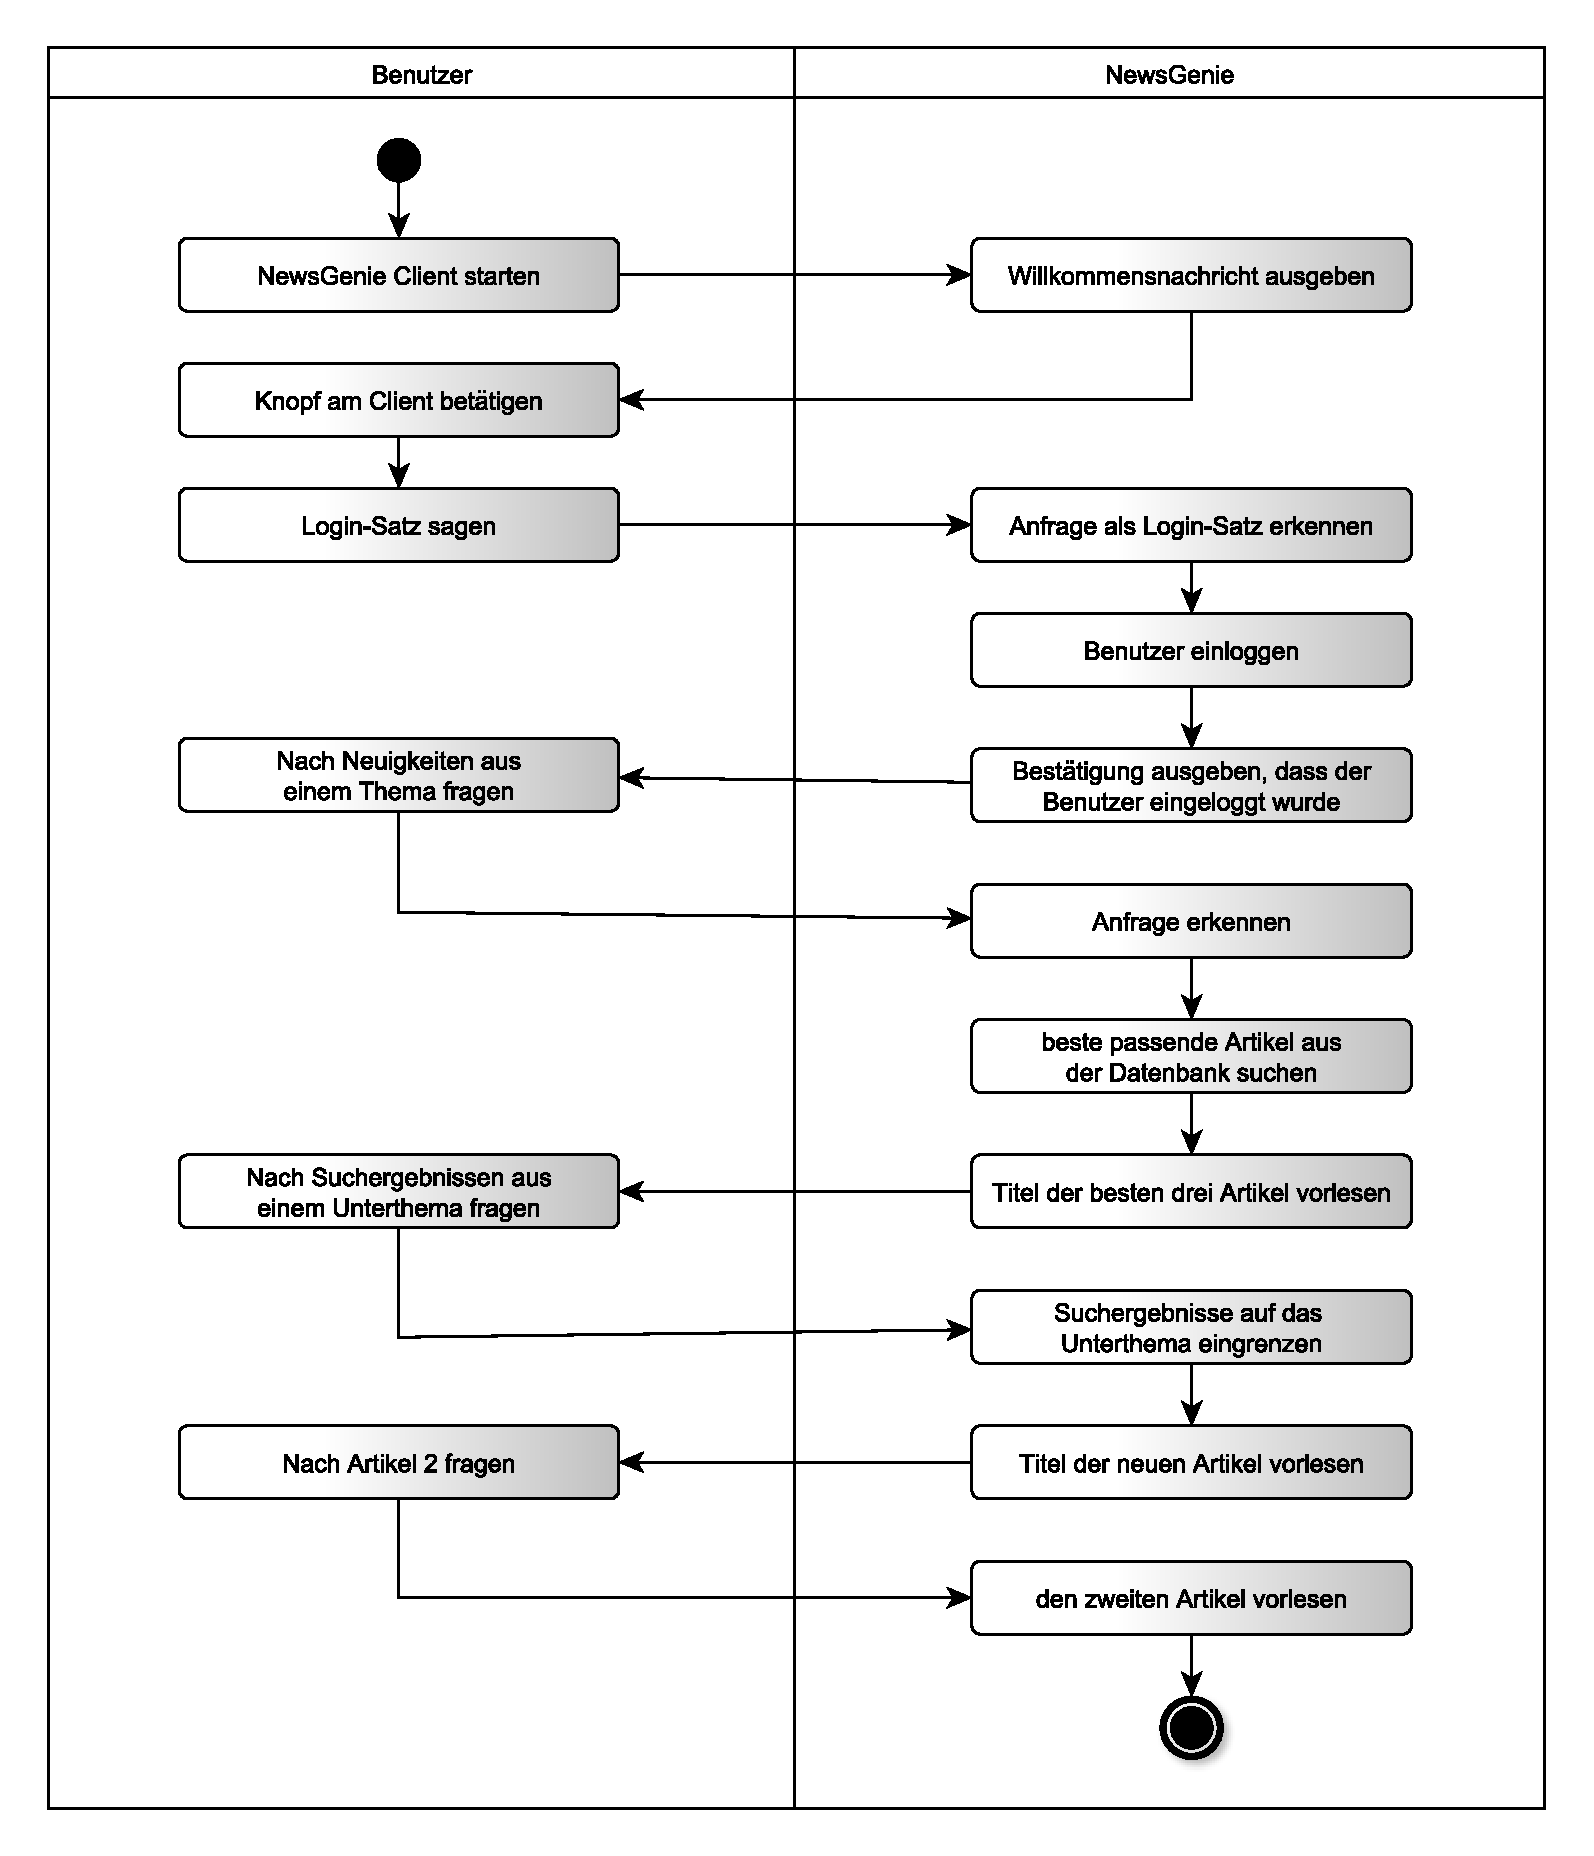
\includegraphics[width=1\textwidth]{Systementwurf/01_einleitung/conversation.eps}
\caption{Aktivitätsdiagramm, \textit{Beispielhafte Kommunikation mit dem Client}
\label{1.5}}
\end{figure}

\begin{figure}[h]
\centering
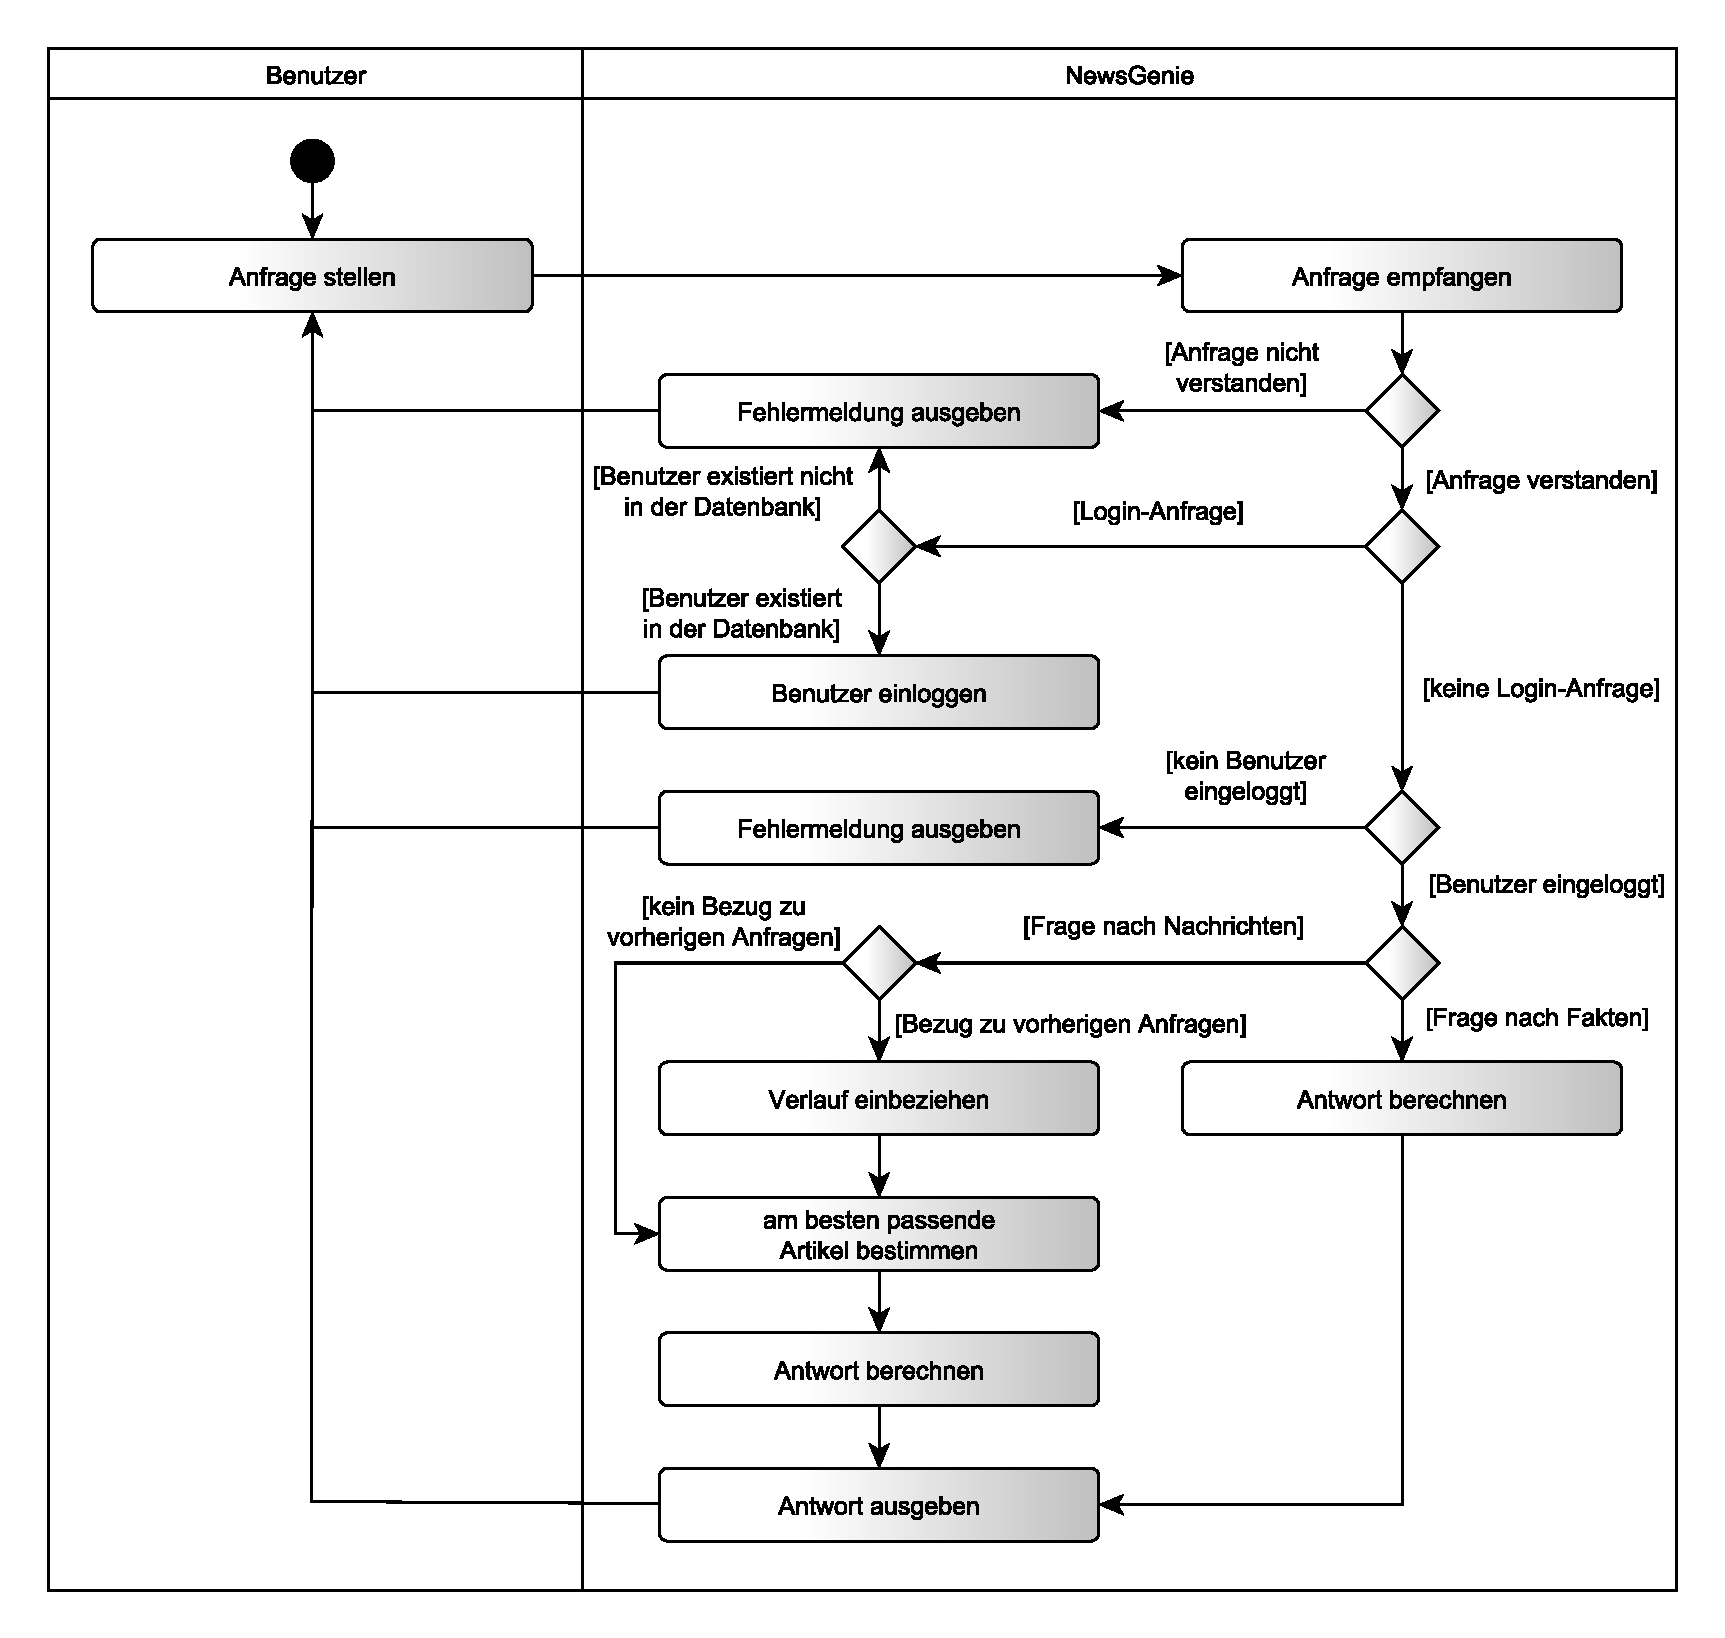
\includegraphics[width=1\textwidth]{Systementwurf/01_einleitung/request.eps}
\caption{Aktivitätsdiagramm, \textit{Verarbeitung einer Anfrage}
\label{1.6}}
\end{figure}

\iffalse
Die zwei Aktivitätsdiagramme in Abbildung \todo[inline]{Referenz} und
\todo[inline]{Referenz} zeigen den Workflow von \NewsGenies Hauptaufgabe, dem
Stellen einer Anfrage an das System.
Hierbei wird vorausgesetzt, dass sich der Nutzer bereits registriert und
entweder (je nach Anfragetyp) am Client oder im Webinterface angemeldet hat.
Will der Nutzer nun eine Anfrage am Client an \NewsGenie stellen, so spricht er
seine Frage. Die Anfrage durchläuft das System und eine Antwort wird
anschließend durch den Client ausgegeben. Dabei hängt die Antwort von dem
Ergebnis der Speech-To-Text- und der eigenen Analyse ab. Kann \NewsGenie zum
Beispiel keine Eingabe bzw. Frage feststellen, so gibt er eine entsprechende
Antwort mit Aufforderung zur Wiederholung der Eingabe auf.
Will der Nutzer stattdessen eine Anfrage im Webinterface an \NewsGenie stellen,
so tippt er seine Frage in das entsprechende Textfeld seine Frage. Nach dem
Klicken auf den "`Ask"'-Button, durchläuft die Anfrage genauso wie beim Client
das System und eine Antwort wird anschließend durch den Client ausgegeben.
Allerdings ist die Wahrscheinlichtkeit einer erfolgreichen Frage hier höher, da
Speech-To-Text hier nicht gebraucht und so die Fehlerwahrscheinlichkeit
minimiert wird.


\todo[inline]{Diagramm 1 - Client}
\todo[inline]{Diagramm 2 - Webinterface}
\fi
%!TEX root = ../Angebot.tex

\chapter{Formale Grundlagen}


Das Back-End der Software wird in der Programmiersprache Java entwickelt. Zur Erstellung der grafischen Schnittstelle des Front-Ends wird die Skriptsrache JavaScript und die textbasierte Auszeichnungssprache HTML 5.0 verwendet.
Diese Aspekte werden in Punkt 5, den Entwicklungsrichtlinien dieses Dokumentes, detailierter aufgef\"uhrt.

Die in der Anwendung verwendete Sprache ist Englisch.
%!TEX root = ../Angebot.tex

\chapter{Projektablauf}

\section{Meilensteine}

Alle wichtigen Ereignisse, wie zum Beispiel Abgabefristen die vom Kunden oder der Projektleitung gesetzt werden, aber auch intern im Team gesetzte Fristen, werden 
in Meilensteinen zusammengefasst und in einer Tabelle wiedergegeben. Dabei ist bei jedem einzelnen Meilenstein jeweils die Vervollst\"andigung gemeint.
Jedes Dokument wird vor jeder offiziellen Abgabe dem Betreuer zur Kontrolle vorgelegt.

\begin{longtable}{|l|c|c|c|c|}
	\hline
	\textbf{Nummer} & \textbf{Meilenstein} & \textbf{Dokumente} & \textbf{Abgabetermin}\\ 
	\hline
	1  	&  Projektstart      &         -     &    13.04.15     \\ 
	\hline
	2	&  Angebot an Betreuer & Angebot & 20.04.15 \\
	 \hline
	3	& Serverapplikation initialisiert & - & 24.04.15 \\
	\hline
	4	& Angebot \"uber Redmine & Angebot & 24.04.15 \\
	\hline
	5	& Vervollst\"andigen der Spielidee &  - & 24.04.15 \\
	\hline
	6 	& Pflichtenheft an Betreuer &  Pflichtenheft & 06.05.15 \\ 
	\hline
	7 	& GUI des Front-Ends  & - & 07.05.15 \\
	\hline
	8 	& Userverwaltung & - & 07.05.15 \\
	\hline
	9 	& Pflichtenheft \"uber Redmine &  Pflichtenheft & 13.05.15 \\
	\hline
	10 	& Zwischenpr\"asentation  &  - & 15.05.15 \\
	\hline
	11 	& Fachentwurf an Betreuer &  Fachentwurf & 27.05.15 \\
	\hline
	12 	& Fachentwurf \"uber Redmine &  Fachentwurf & 03.06.15 \\	
	\hline
	13 	& Verwaltung f\"ur Benutzerrechte & - & 24.06.15 \\
	\hline
	14 	& Technischer Entwurf an Betreuer &  Technischer Entwurf & 24.06.15 \\
	\hline
	15 	& Softwaretests & - & 30.06.15 \\
	\hline
	16 	& Technischer Entwurf \"uber Redmine &  Technischer Entwurf & 01.07.15 \\
	\hline
	17 	& Fertigstellung Minigame & - & 24.06.15 \\
	\hline
	18 	& Testdokumentation an Betreuer &  Testdokumentation & 08.07.15 \\
	\hline
	19 	& Testdokumentation \"uber Redmine &  Testdokumentation & 15.07.15 \\
	\hline
	20 	& Pr\"asentationsvorbereitung & - & 20.07.15 \\
	\hline
	21 	& Fertige Version &  Quellcode, ... & 23.07.15 \\
	\hline
\end{longtable}

\section{Geplanter Ablauf}

Ein Teil des Teams startet das Projekt mit dem Ausformulieren des Produktangebots. W\"ahrenddessen beginnt das Gestaltungsteam ihren kreativen Prozess.
Ideenentwicklung und -austausch sowie N\"utzlichkeitsabw\"agung f\"uhren schnell zur fertigen Spielidee. Dieser Ablauf wird gleichzeitig genutzt, um zu pr\"ufen welche 
Werkzeuge (Frameworks, Entwicklungsumgebungen, etc.) genutzt werden, und sich mit diesen vertraut zu machen. Dabei werden auch schon erste Grafiken wie etwa 
f\"ur den Start-Screen und das Hauptmen\"u enstehen.

Das Back-End-Team nutzt die Zeit um die Serverapplikation zu erstellen. Desweiteren werden Ideen f\"ur ein Administrationstool sowie zur User- und Datenverwaltung 
gesammelt und umsetzbar strukturiert. Zwischenzeitig wird ein Papierprototyp entstehen, der die Grundz\"uge der zu erstellenden Applikation enth\"alt und das Team auf
einen gemeinsamen Stand bringt.

Sobald der Kunde, sowie der Betreuer das Angebot angenommen haben, beginnt der praktische Teil.

Das n\"achste Ziel wird sein, einen lauff\"ahigen Prototypen zu entwickeln.
Daf\"ur erstellen ausgew\"ahlte Mitglieder des Entwicklerteams das sogenannte Pflichtenheft, um festzuhalten, was von dem Projektteam alles geliefert werden muss.
Bis zur Fertigstellung des Prototypen und dessen Pr\"asentation wird weiterhin ein Fachentwurf erstellt und eingereicht.

Das Front-End-Team wird nun sowohl das Hauptmen\"u als auch das \glqq Alchemistenlabor\grqq~(den eigentlichen \glqq SQL-Vokabeltrainer\grqq) bearbeiten, damit der repr\"asentative 
Teil des Projekts m\"oglichst zur Zwischenpr\"asentation ausf\"uhrbar ist.
Parallel wird sich das Back-End-Team um die Nutzer- und Rechteverwaltung k\"ummern. 

Nach der Zwischenpr\"asentation werden der Projektdokumentation noch der Technische Entwurf und die Testprotokolle hinzugef\"ugt.
Um die dazugeh\"origen Software-Tests k\"ummert sich das Team in der letzten Etappe.

Zum Abschluss des Projektes wird eine kleinere Gruppe aus ausgew\"ahlten Mitgliedern noch f\"ur eine gute Pr\"asentation beim Tag der jungen Software-Entwickler 
(TDSE)  sorgen. 

Zur besseren \"Ubersicht dieser einzelnen Abl\"aufe ist ein Gantt-Diagramm erstellt worden.

\begin{figure}[ht]
\centering
\includegraphics[height=\textwidth, angle=90]{figures/gantt.pdf}
\caption{Gantt-Diagramm}
\label{gantt}
\end{figure}
%!TEX root = ../Angebot.tex

% Kapitel 4
%-------------------------------------------------------------------------------

\chapter{Projektumfang}

\section{Lieferumfang}

Zum Lieferumfang der Software geh\"oren:

\begin{itemize}
	\item der Quellcode des Programms
	\item die ausf\"uhrbare Software
	\item die hinter der Nutzerschnittstelle liegende Datenbank
	\item das zugeh\"origes Handbuch
	\item die Spezifikation und der Entwurf der Software
	\item die Protokolle der Tests
	
\end{itemize}

\section{Kostenplan}

Die f\"ur das Projekt anfallenden Kosten, werden auf ca. 316.000 Euro gesch\"atzt. Davon entfallen
315.000 Euro auf den Lohn der Projektmitglieder (ausgehend von einem Arbeitslohn von 100 Euro pro Stunde und 30 Arbeitsstunden je Mitglied) 
und 1000 Euro auf den Kauf von Sprites, vorgefertigten Spieleger\"usten und weiteren f\"ur das Spiel ben\"otigten Objekten.

\section{Funktionaler Umfang}

Folgende Funktionen sollen in der abschlie{\ss}enden Version der Software enthalten sein:
\begin{enumerate}
	\item Insgesamt soll das Spiel dem Nutzer 3, beziehungsweise 4 verschiedene Modi bieten:
	\begin{enumerate}
      		\item Einen narrativen Modus, welcher dem Spieler erm\"oglicht in der Rolle des Alchemisten verschiedene Aufgaben zu 
			 erf\"ullen, um dann in der Geschichte des Spiels voranzuschreiten. Wobei es unabdingbar ist, dass der User
			 SQL-Anfragen \"ubt um in dem Modus weiter zu kommen.
		\item Einen Trivia-Modus, durch den die Spieler abseits eines festgelegten Handlungsstranges SQL-Abfragen \"uben 
			 k\"onnen,	indem sie zuf\"allig gestellte Aufgaben l\"osen.
		\item Einen Sandbox-Modus, der den Trivia-Modus durch vom Nutzer selbst erstellte Aufgaben erweitert. Diese Aufgaben 
			 stehen dann allen Nutzern zur Verf\"ugung und k\"onnen bewertet werden. Das Erstellen von Aufgaben jedoch bleibt freigeschalteten Spielern 
			 vorenthalten die sich im narrativen Modus bew\"ahrt haben. Dies wir durch das Back-End mit bestimmter Rechteverwaltung
			 realisiert.
		\item Einen Season-Modus, welcher von den Dozenten des Studienfaches RDBI genutzt werden kann, um die Software in den 
			 \"Ubungsbetrieb zu integrieren.
	\end{enumerate}
	\item Nutzerprofile und -statistiken, die den Fortschritt und die Erfolge eines jeden Spielers speichern. Au{\ss}erdem sollen diese grafisch
		aufbereitet werden und von jedem User abrufbar sein.
	\item Ranglisten, \"uber die sich die Nutzer untereinander vergleichen k\"onnen um die Motivation zu f\"ordern. 
		 Eventuell ist die Nutzung angemeldeten Spielern vorbehalten. 
	\item Ein Minispiel, welches sowohl im Story-, als auch im Trivia-Modus zum Einsatz kommt. Dabei handelt es sich um ein 
		 \glqq Jump \& Run\grqq-Spiel, in welchem die Spieler Gegenst\"ande einsammeln um Punkte zu erhalten und dabei 
		 SQL-Hindernisse \"uberwinden m\"ussen.
	\item Eine Benutzerverwaltung, die einzelne Rechte, sowie Rollen verwalten soll.
	\item Ein Admin-Tool, damit Dozenten und deren Mitarbeiter die Software in 
   		 ihre \"Ubungen integrieren k\"onnen. Insbesondere die Challenges, in dem Fall die Hausaufgaben, sollen hiermit erstellt und 
		 eingepflegt werden k\"onnen. Beim Erstellen von Hausaufgaben kann man einen Titel ausw\"ahlen und andere Eigenschaften
		 festsetzten. Zum Beispiel kann ein Zeit-Slot gesetzt werden in der die Hausaufgabe bearbeitet werden muss. 
	\item Auch die Studenten k\"onnen im Anschluss der Bearbeitung dieses Tool nutzen um zu \"uberpr\"ufen
		 ob sie die Hausaufgaben bestanden haben oder nicht. 
	\item Das Back-End bietet ebenfalls eine Schnittstelle an, die mit dem Software-Modul des Teamprojektes kommuniziert und es mit 
		entsprechenden XML-Schemata f\"ullt.
	\item Die Studenten bekommen die M\"oglichkeit Kommentare zu den Hausaufgaben abzugeben. Somit bekommt auch der Betreuer der
		Hausaufgaben eine Rewiew zum Schwierigkeitsgrad oder \"ahnlichen Kriterien. Auch dies wird durch das Back-End verwaltet.
\end{enumerate}




%!TEX root = ../Angebot.tex

\chapter{Entwicklungsrichtlinien}

\section{Konfigurationsmanagement}

Es gibt ein zentrales Repository auf Basis von Subversion (SVN), welches \"uber das Redmine des Instituts f\"ur Softwaretechnik und Fahrzeuginformatik (ISF) zur Verf\"ugung gestellt wird. Dieses Repository ist in drei Ordner unterteilt. In einem Ordner werden alle im Laufe des Projektes zu angefertigten Dokumente, die die Projektorganisation und den Kunden betreffen, abgelegt. Dazu z\"ahlen: ein Fachentwurf, eine Abnahmespezifikation, ein Pflichtenheft, ein technischer Entwurf, eine Testspezifikation und die entsprechenden Testprotokolle. Au{\ss}erdem gibt es zwei weitere Ordner, in die alle Dateien der jeweiligen Teilprojekte, das Back- sowie das Front-End, abgelegt werden. Hierbei handelt es sich unter anderem um Dateien mit dem Quellcode der jeweiligen Software-Komponente.  

Des Weiteren gibt es eine feste Kommentarstruktur, die bei jedem SVN-Commit, also dem Hochladen der ge\"anderten Dateien in das SVN-Repository, eingehalten werden soll. Dies f\"uhrt dazu, dass alle \"Anderungen nachvollziehbar, verst\"andlich und vollst\"andig sind. Um die Integrit\"at der Applikation zu gew\"ahrleisten, soll ebenfalls nur vollst\"andig ausf\"uhrbarer Code in das Repository hochgeladen werden.  


\section{Design- und Programmierrichtlinien}

F\"ur die Entwicklung des gesamten Projektes ist festgelegt, dass sich die Entwickler an folgende im Rahmen der Veranstaltung \glqq Software-Engineering I (SE I)\grqq~vorgestellten Coding-Guidelines halten:
\begin{itemize}
	\item Einr\"uckung: Um den Code \"ubersichtlicher zu gestalten, wird die Einr\"uckungstiefe auf 4 Zeichen festgelegt.
	\item Klammersetzung: Jede Klammer die zur Schlie{\ss}ung einer Methode bzw. einer Klasse gebraucht wird, wird in eine neue Zeile gesetzt. 
	\item Bezeichner: S\"amtliche Bezeichener (Parameter, Variablennnamen, Methodennamen, Klassennamen, etc.) werden sinnvoll nach ihrem Inhalt 		bennant, damit direkt ersichtlich ist, was die jeweilige Methode berechnet oder welche Information in jeder Variable steht.
	\item CamelCaseNotation: Zur besseren Lesbarkeit des Quelltextes werden Methoden in CamelCaseNotation notiert. 
	\item UPPER\_CASE Notation: Alle Konstanten werden in Gro{\ss}buchstaben, durch Unterstriche getrennt, geschrieben.
	\item lower\_case Notation: Imports und Packages werden in Kleinbuchstaben geschrieben.	
\end{itemize} 

Dar\"uber hinaus ist entschieden, s\"amtliche Kommentare auf Englisch zu verfassen.
Das Software-Dokumentationswerkzeug Javadoc generiert parallel aus dem Java-Quellcode eine vollst\"andige HTML-Dokumentationsdatei.

%!(Bestandteil des Java Development Kits) glossar


\section{Verwendete Software}

Als Entwicklungsumgebung wird IntelliJ IDEA von JetBrains verwendet, zum Erstellen von Diagrammen und technischen Zeichnungen  das Visualisierungsprogramm Dia, sowie Microsoft Visio. Textdokumente, die das Projekt betreffen, werden mit Hilfe des Software-Pakets LaTeX angefertigt und formatiert.

Das Front-End wird mithilfe der HTML5 Spiele-Engine melonJS und der plattformunabh\"angigen JavaScript-Bibliothek jQuery entwickelt, das Admin-Tool des Back-Ends mit dem Open-Source-Framework AngularJS und dem CSS-Framework Bootstrap.
F\"ur die Server-Komponente des Back-Ends wird das Web-Framework play! verwendet. 

Das Front-End-Team nutzt f\"ur das zu entwickelnde Mini-Spiel den Tiled Map Editor. Grafiken f\"ur die gesamte Software werden mit Hilfe des Bildbearbeitungsprogramm Adobe Photoshop CS6 entstehen.

Au{\ss}erdem wird eine Software des mitarbeitenden Teamprojektes, die automatisch Schemata generiert zur Verf\"ugung gestellt. Zudem kann auf eine Software, die im Rahmen einer Bachelorarbeit entwickelt wird, zur\"uckgegriffen werden, die sich mit der automatischen Generierung von SQL-Statements und Aufgabenstellungen besch\"aftigt.




%!TEX root = ../Angebot.tex

\chapter{Projektorganisation}

\section{Schnittstelle zum Auftraggeber}

Der Kunde steht den Entwicklern per Telefon-, E-Mail- und pers\"onlicher Kommunikation zur Verf\"ugung. Regelm\"a{\ss}ige
Meetings wurden direkt zu Anfang des Projektes auf donnerstags um 15 Uhr festgelegt.


\section{Schnittstelle zu anderen Projekten}

Die Mitglieder des externen Teamprojektes, die ihre Software zur Verf\"ugung stellen, und der Verfasser 
der Bachelorarbeit, dessen Software ebenfalls zur Verg\"ugung gestellt wird, k\"onnen sowohl \"uber die 
Projektbetreuer, als auch per E-Mail erreicht werden. 
Der Datenaustausch geschieht hierbei \"uber GitHub.

\section{Interne Kommunikation}

Das SEP-Team kommuniziert \"uber E-Mail bzw. Instant-Messenger und das eingerichtete Repository im Redmine.
Au{\ss}erdem finden sowohl mit den Betreuern und dem Kunden, als auch intern untereinander regelm\"a{\ss}ige Treffen statt.
Die Treffen werden mit dem Online-Termin-Planer Doodle organisiert.
Zur Protokollierung dieser Meetings wird ein webbasierter Editor von Google verwendet.


%\section{Kontaktdaten}

	
	
%!TEX root = ../Angebot.tex

\chapter{Glossar}

\begin{itemize}
	\item Back-End: Das Back-End bezeichnet eine Schicht eines Programms. Das Back-End verarbeitet zur Verf\"ugung gestellte Daten. Es entspricht hierbei der Serverkomponente des Programms.
	\item Front-End: Das Front-End ist das Gegenst\"uck zu dem Back-End. Es beschreibt Ausgabe des Programms und ist f\"ur eine entsprechende Visualisierung zust\"andig.
	\item Javadoc: Javadoc ist ein Software-Dokumentationswerkzeug, das aus Java-Quelltexten automatisch HTML- Dokumentationsdateien erstellt. 
	\item Redmine: Das Redmine ist eine webbasierte Organisations- und Projektverwaltungssoftware.
	%!\item Sprite: Ein Sprite ist ein zweidimensionales Grafikobjet. 
	\item Repository: Ein Repository ist ein verwaltetes Verzeichnis zur Speicherung von Daten
	\item Framework: Ein Framework ist ein vorgefertigtes Programmierger\"ust.
	\item Spiele-Engine: Eine Spiel-Engine ist ein spezielles Spiele-Framework, das den Spielverlauf steuert und f\"ur die Visualisierung des Spiels sorgt.  
\end{itemize}







%------Ende des Dokumentes------------------------------------------------------
\end{document}
